
\begin{equation}\label{Somireddy}
\bar{\sigma}_{ij}=\frac{1}{V_{RVE}}\int_V \sigma_{ij}(x_1,x_2,x_3)dV \end{equation}

\begin{equation}\label{Somireddy2}
\bar{\epsilon}_{ij}=\frac{1}{V_{RVE}}\int_V \epsilon_{ij}(x_1,x_2,x_3)dV
\end{equation}

%The strain energy $U*$ in the heterogeneous volume of the RVE is computed by:
\begin{equation}\label{Strainenergy}
U^*=\frac{1}{2} \int_{V_{RVE}} \sigma_{ij} \epsilon_{ij} dV
\end{equation}

%And the strain energy calculated for homogeneous RVE using homogenized modulus is

\begin{equation}\label{Strainenergy2}
U=\frac{1}{2} \sigma_{ij} \epsilon_{ij} V_{RVE}
\end{equation}

%The general idea of homogenization model is to find globally homogeneous medium equivalent to the original microscopically heterogeneous material, where the strain energy stored in both systems is approximately same, that means $U^*=U$. 

%This results in the equation
\begin{equation}\label{Strainenergy3}
U^*=\frac{1}{2} \bar{\epsilon}^T |C| \bar{\epsilon}^T V_{RVE}
\end{equation}

%The unknown elements in the constitutive matrix can be calculated by solving for different load cases. The strain energy ($U^*$) of a deformation mode is obtained by employing a FEM simulation using equation \ref{Strainenergy3} and consequently the corresponding unknown stiffness of the constitutive matrix is calculated. The average strains are obtained from applied boundary displacements ($U_i$) on the RVE and the average strains in equation \ref{Strainenergy2} can be converted as 

\begin{equation}\label{averagestrains}
\bar{\epsilon}_{ij}=\frac{1}{V_{RVE}}\int_{S_1} (u_i n_j+u_j n_i) dV
\end{equation}

%Since the RVE is supposed to be continuous in a physical body, the RVE is subjected to periodic boundary conditions which represent the continuous nature of the larger solid. The displacement field of the RVE can be expressed as:
\begin{equation}\label{displacementfield}
u_1(x_1, x_2, x_3)=\bar{\epsilon}_{ik} (x_k +u_i^*x_1 x_2 x_3)
\end{equation}

\begin{figure}[H]
    \centering
    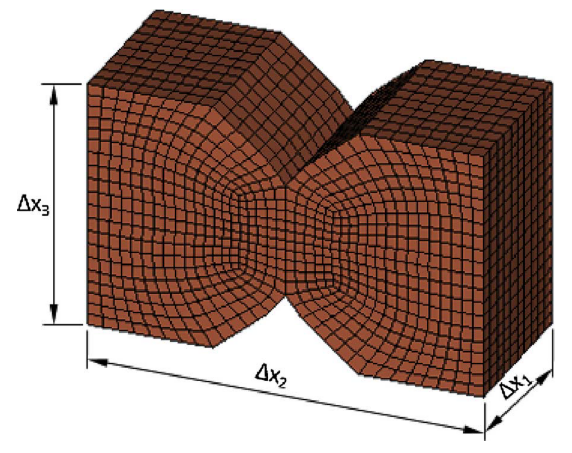
\includegraphics[width=0.5\textwidth]{chapter_2/figures/RVEsomireddy.PNG}
    \caption{Meshed RVE by Somireddy}
    \cite{Somireddy2018DevelopmentFDM}
    \label{fig:Homogenization}
\end{figure}

%Where $\bar{\epsilon}_{ik}$ is the average strains tensor and the first term on the right side of equation \ref{displacementfield} represents a linear distributed displacement field. $u_i^*x_1 x_2 x_3$ represents the periodic function from one RVE to another. This function is in \ref{displacementfield} unknown and therefore, the displacement cannot be directly applied to boundaries of the RVE. These boundary conditions are suitable for parallelepiped RVE models. The displacements are related between different RVE's via their boundary nodes due to the periodic nature of the larger geometry. The equations that are implemented are easily applicable to FE models as a nodal displacement constraint and also guarantee traction continuity condition along with displacement continuity for a periodic RVE Model.

%This process is explained in detail by Zhang \cite{XiaAApplications} for orthotropic composites and implemented by Somireddy \cite{Somireddy2018DevelopmentFDM} for FFF RVE's.

When applying the classical laminate theory we must consider the global coordinate system (x,y,z) for a laminate plate, and local coordinate system (1,2,3) for a lamina. The properties of the rotated ply can be calculated by multiplying with the so called transformation matrix. 
\begin{equation}\label{Transformation matrix}
T=\begin{vmatrix}
c^2 & s^2 & 2cs\\
s^2 & c^2 & -2cs \\
-cs & cs & c^2-s^2\\
\end{vmatrix}
\end{equation}
Where $c=cos\theta$  and $s=sin\theta$. Then the stresses in global coordinates for each ply k become:
\begin{equation}\label{CLT}
\begin{vmatrix}
\sigma_{xx}\\
\sigma_{yy}\\
\sigma_{xy}\\
\end{vmatrix}^{(k)}
= (|T|^{(k)})^{-1}|Q|^{(k)}|T|^{(k)}
\begin{vmatrix}
\epsilon_x_x\\
\epsilon_y_y\\
\epsilon_x_y\\
\end{vmatrix}^{(k)}
\end{equation}

This can be simplified to a adjusted stiffness matrix $|\bar{Q}|^{(k)}$ for the calculation of stresses in global system. From the definition of strains found according to the Classical Plate Theory \cite{Ishai2006EngineeringMaterials} the stresses at each ply can be obtained by:

\begin{equation}\label{CPT}
\{\sigma\}^{(k)}=|\bar{Q}|^{(k)}\{\epsilon^0\}+|\bar{Q}|^{(k)}z\{\kappa^0\}
\end{equation}

Where z is the distance from the mid-plane in the direction perpendicular to the mid-plane itself, $\{\epsilon^0\}$ are the midplane strains, and $\{\kappa^0\}$ are the mid-plane curvatures as can be seen in figure \ref{fig:Midplane}. 

\begin{figure}[H]
    \centering
    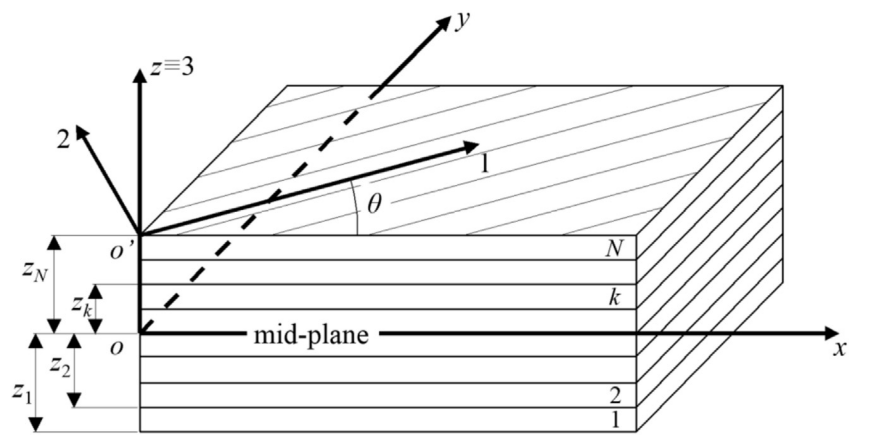
\includegraphics[width=0.75\textwidth]{chapter_2/figures/Midplane.PNG}
    \caption{Globalcoordinate system \{O,x,y,z\} for the laminate and material coordinate systems \{0',1,2,3\} for the laminas} \cite{Alaimo2017InfluenceParts}
    \label{fig:Midplane}
\end{figure}


%Add relation A and Q----

The laminate normal and shear forces, $N_x, N_y, N_x_y$ are related to mid-plane strains and curvatures through the following expressions:
\begin{equation}\label{normalforces}
\begin{vmatrix}
N_x\\
N_y\\
N_x_y\\
\end{vmatrix}^{(k)}
= |A| \{\epsilon^0\} + |B| \{\kappa^0\}
\end{equation}

While laminate bending and twisting moments $M_x, M_y, M_x_y$ are related to strains and curvatures as shown below:

\begin{equation}\label{Bending}
\begin{vmatrix}
M_x\\
M_y\\
M_x_y\\
\end{vmatrix}^{(k)}
= |B| \{\epsilon^0\} + |D| \{\kappa^0\}
\end{equation}

Where the A, B and D matrices are calculated as follows:
\begin{equation}\label{A}
A_i_j=\sum_{k=1}^{Nplies} \bar{Q}^{(k)}_{ij} (z_k-z_{k-1})
\end{equation}
\begin{equation}\label{B}
B_i_j=1/2\sum_{k=1}^{Nplies} \bar{Q}^{(k)}_{ij} (z^2_k-z^2_{k-1})
\end{equation}
\begin{equation}\label{D}
D_i_j=1/3\sum_{k=1}^{Nplies} \bar{Q}^{(k)}_{ij} (z^3_k-z^3_{k-1})
\end{equation}
Plastic and failure modelling}
There exists several yield and failure criteria for thermosets and composites. Since thermpolastics have a more complex behaviour due to their viscoeleasticity in this section the different models will be discussed. 
Lin\cite{Lin2013StressLoading} confirms the lack of accurate yielding and failure criteria for thermoplastics. Additionally, the PhD. thesis of Melick \cite{Melick2002DeformationGlasses} on the deformation and fracture of polymer glasses also mention the lack of failure criterion, and does not produce a satisfying solution for tis issue. Different  models (brittle or ductile) are implemented in commercial software sucha as the equivalent strain criterion, von Mises, Johnson-Cook, Hill and Drucker-Prager. The main drawback in these fracture models is that accurate predictions of failure can only be achieved for limited stress state and strain rate, which cannot be applied for thermoplastics. One of the currently popular material models for polymer plasticity  in LS-DYNA is SAMP-1 (semi analytical model for polymers)

\subsubsection{Yield}
The yield criteria for Polymer Materials proposed by Hilary\cite{Halary2011PolymerMaterials} is defined in equation \ref{eqn:yieldpolymers}. The resulting yield surface is shown in figure \ref{fig:yieldpolymers}

\begin{figure}[H]
    \centering
    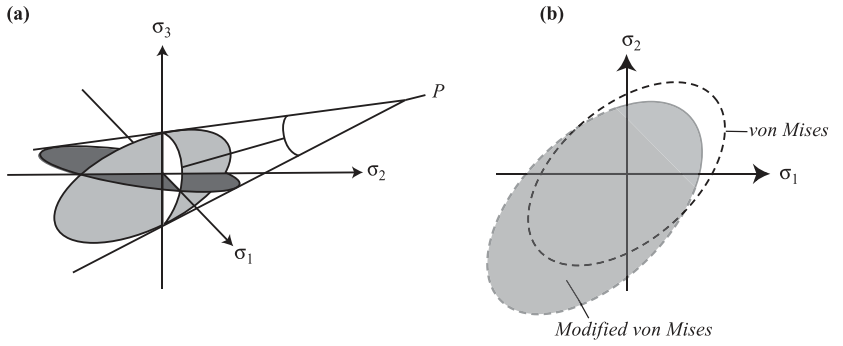
\includegraphics[width=0.75\textwidth]{chapter_2/figures/yieldpolymers.png}
    \caption{Yield surface for polymers a) three-dimensional b) two-dimensional compared with von Mises \cite{Halary2011PolymerMaterials} }
    \label{fig:Midplane}
\end{figure}
Melro proposes a paraboloidal yield criterion for epoxies defined by Tschoegl, which can be defined as:
\begin{equation}\label{AzziTsai}
\Phi=6J_2+2I_1(\sigma_c-\sigma_t)-2\sigma_c\sigma_t
\end{equation}Where $J_2$ is the second invariant of the deviatoric stress tensor, and $I_1$ = tr(\textbf{$\sigma$})

Du Bois \cite{DuBois2006APolymers} implemented a seminanalytical model for the simulation of polymers (SAMP-1) in LS-DYNA under MAT187. This is currently quite popular,  using a different yield surface.
\begin{equation}\label{AzziTsai}
f=\sigma_v^2-A_0-A_1*\sigma_h-A_2*p^2<0
\end{equation}For further details the reader is referred to the mentioned article. 

Another popular yield criterion that is used by the SAMP-1 material model in LS-DYNA is that Drucker-Prager yield criterion. 

\subsubsection{Failure and damage}
In FEM modelling software different damage and failure models are implemented. The damage initiation point defines the point of initiation of degradation of stiffness, it only leads to effective damage if damage evolution is specified \cite{ABAQUS2006MaterialFailure}. In case of ductile damage, D is rather a function of plastic straining and affect the yield stress rather than the elastic modulus. This is equivalent to plastic softening. The material point is assumed to fail when the overall damage variable D reaches a critical value $D_{max}$.
A general form of the strain based fracture loci for thermoplastics can be written as follows
\begin{equation}\label{AzziTsai}
\bar{\epsilon_f}=f(\eta)=f(\frac{\sigma_h}{\sigma_v})
\end{equation}
%In the SAMP-1 a simple damage model was added where the damage parameter D is a function of plastic strain only. In this model a load cuve must be provided by the user giving D as a function of the plastic strain under uniaxial tension. The value of the critical damage $D_c$ leading to rupture is then the only other required additional input, this model behaves istropically. Furthermore the model uses the notion of the effective cross section, which is the true cross section of the material minus the cracks that have happened. 
%This models assumes the start of damage from the yield point, and fails when the damage parameter D drops to 0.   

One of the most popular fracture and damage models for polymers is the Johnson Cook model, widely applicated in ABAQUS and LS-DYNA softaware:

\begin{equation}\label{AzziTsai}
\epsilon_f=(d_1+d_2*exp{(d_3*\frac{\sigma_h}{\sigma_v})}*(1+d_4*\frac{\dot{\epsilon}}{\dot{\epsilon}})
\end{equation}
Where $d_i$ are material parameters\cite{BoisA:}, the Hancock-McKenzie defines the following parameters: $d_1=0, d_2=3/2, d_3=\epsilon_{1f}*exp(-1/2)$. Additionally, a paper by Gao \cite{Gao2013CriticalPipelines} proposes a different variant of the Johnson Cook criterion:

\begin{equation}\label{AzziTsai}
\epsilon_{fp}=1.65\epsilon_{1fp}{(-\frac{3}{2}*\frac{\sigma_h}{\sigma_v})}
\end{equation}Where $\epsilon_{1f}$ is the critical strain for ductile materials at which crack are initiated under tension. Different strain based failure criteriona are proposed in LS-DYNA and abaqus. Most implement a simple plastic strain at failure ($\epsilon_p<\epsilon_{pf}$) or a major strain failure ($\epsilon_1<\epsilon_{1f}$), and others use the Johnson-Cook criterion as is described.  

Damage in combination with the Johnson Cook model is defined in material model SAMP-1 in LS-DYNA as:

\begin{equation}\label{AzziTsai}
d=\epsilon_p/\epsilon_f\Rightarrow d<d_c\Rightarrow\epsilon_p<\epsilon_{pf}=d_c*\epsilon_f
\end{equation}The influence of stress triaxiality in a strain based failure criterion is important because different states of stress would result in a different equivalent strain at failure\cite{BoisA:}. 
%damage in polymers
A damage variable, denoted as D, quantifies the part of the material cross section that no longer transmits forces (cracks or voids). In the following, only isotropic damage is considered. Elastic damage affects material stiffness, ductile damage affects material strenght or both material strength and stiffness. This depends on the chosen formulation where two different approaches may be postulated: strain equivalence or energy equivalence. We will be discussing strain equivalence in this section. 

Damage in polymers is relatively hard to model, since different mechanisms play a large role in the determination of damage. A study on the damage behaviour of polymers \cite{Gu2013ExperimentalThermoplastics}, Gu et al. presents different damage functions based on literature and proposes damage functions based on experimental data. 
The general stiffness damage as function of plastic strain is defined as

\begin{equation}\label{stiffnessdamage}
E_{eff}=E_0*(1-d)
\end{equation}Where Nutini and Vitali proposed a simple definition of the damage parameter calculated from the volume strain, since an important characteristic of thermoplastics is the generation of damage (voids and crazes) during plastic volumetric deformation $\epsilon_v$, which is defined as the sum of the principle strains.

\begin{equation}\label{AzziTsai}
d=1-exp(-\epsilon_v)
\end{equation}

In figure \ref{fig:damagepolymer} the results from a loading/unloading experiment was carried out on a polypropylene sample to get more insight on the damage behaviour. 

\begin{figure}[H]
    \centering
    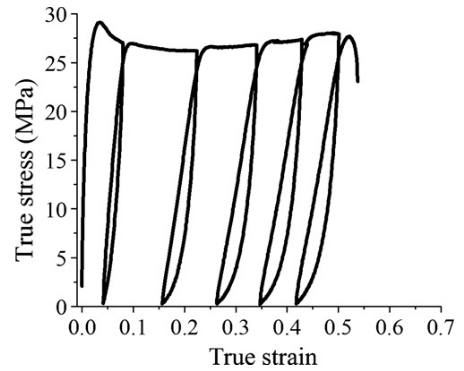
\includegraphics[width=0.4\textwidth]{chapter_2/figures/damagepolymer.png}
    \caption{Sample of trues stress-strain curve of polypropylene\cite{Gu2013ExperimentalThermoplastics} }
    \label{fig:damagepolymer}
\end{figure}
As can be seen, the Youngs modulus is slightly decreases with plastic strain. However, after the first cycle (just after the softening region) the change in stiffness seems minimal.  Unfortunately, no absolute values of the Youngs moduli are presented in this study. 
Following the results, this study proposed a damage function that follows the equation \ref{eqn:stiffnessdamage} fitting the experimental results. Since the damage only occurs in the plastic region for polymers, the result is a function of plastic strain ($\epsilon_p$), and is fitted with a double term exponential function:

\begin{equation}\label{AzziTsai}
d=A*(exp(B*\epsilon_p)-exp(D*\epsilon_p))
\end{equation}The study concludes that the damage parameter calcultated with the volumetric deformation underpredicts the damage occurring. A possible reason is that besides voids and crack that might be captured with the volumetric strain, microscracks that do not lead to macroscopic volume change also contribute to damage. 

Christensen \cite{Christensen2013TheFailure}  published a detailed book on failure criteria, but did not take into account materials that exhibit strain softening, therefore his extensive work can unfortunately not be used. 



Rodriguez \cite{Rodriguez2003MechanicalModeling} investigated yield modelling for composite materials under multi-axial loading. He implemented a theory proposed by Tsai-Hill for composites, which is an extension of the von-mises yield criterion, which defines failure for composites. Originally the Hill theory was developed for anisotropic ductile and brittle materials. Different variations are used for either failure or yield criteria. The  surface is assumed to be quadratic in the stress components. Details on these yield criteria can be found in books on composite mechanical behaviour \cite{Ishai2006EngineeringMaterials}, \cite{Mallick2007Fiber-Composites}.


%________________________

\begin{equation}\label{AzziTsai}
f(\sigma_{ij})=C_1(\sigma_{22}-\sigma_{33})^2+C_2(\sigma_{33}-\sigma_{11})^2+C_3(\sigma_{11}-\sigma_{22})^2
\\
+2C_4\sigma(_{23})^2+2C_5\sigma(_{13})^2+2C_6\sigma(_{12})^2=1 
\end{equation}

where the coefficients $C_1$,$C_2$,$C_3$,$C_4$,$C_5$ and $C_6$ are determined from tensile and shear tests in the axes of anisotropic symmetry. The tensile values must be positive and compressive values must be negative. Since all the terms in equation \ref{AzziTsai} are squared, the failure surface predicts the same strength in tension as in compression. For the case of plane stress in the 1-2 plane of a unidirectional lamina with fibers oriented in direction 1, then $\sigma_{33}=\sigma_{13}=\sigma_{23}$=0. If the transverse strengths of FFF parts are assumed equal (they are different), the failure surface reduces to:

\begin{equation}\label{planestress}
\frac{\sigma_{11}^2}{S_1^2}-\frac{\sigma_{11}\sigma_{22}}{S_1^2}+\frac{\sigma_{22}^2}{S_2^2}+\frac{\sigma_{12}^2}{S_{12}^2}=1
\end{equation}

where $S_1$ is the strength in direction 1 (direction of the fibers), $S_2$ is the strength in the transverse direction and $S_{12}$ is the in-plane shear strength. The components are found when solving the equation for some basic stress states: uniaxial longitudinal, uniaxial transverse, in-plane shear, and biaxial tests, respectively.

Azzi-Tsai-Hill criterion is similar to Tsai-Hill the  criterion, in the way the failure surface is determined. The only difference is that the absolute value of the cross product term is taken. This difference between the two failure criteria shows up only when $\sigma_{11}$ and $\sigma_{22}$ have different signs.

The Tsai-Wu criterion is an extension on the Tsai-Hill criterion. Tsai-Wu uses an additional F12 term that requires a biaxial test, where Tsai-Hill uses the material properteis in the 1 and 2 directions.  

\begin{equation}\label{AzziTsai}
f(\sigma_{ij})=C_1(\sigma_{22}-\sigma_{33})^2+C_2(\sigma_{33}-\sigma_{11})^2+C_3(\sigma_{11}-\sigma_{22})^2
\\
+2C_4\sigma(_{23})^2+2C_5\sigma(_{13})^2+2C_6\sigma(_{12})^2=1 
\end{equation}
\begin{figure}[H]
    \centering
    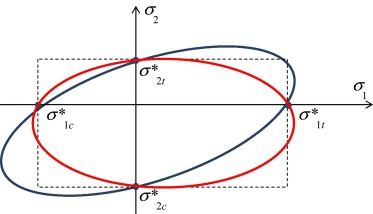
\includegraphics[width=0.5\textwidth]{chapter_2/figures/Tsaiandwu.jpg}
    \caption{Tsai-Wu (blue) vs Tsa-Hill (red)failure surface }
    \cite{Sheth2017NumericalOrientation}
    \label{fig:RVESheth}
\end{figure}

Since our goal is to model an RVE that implement the properties of bulk material (ABS) it would be more important to find a criteria for this material. 
%strain based fracture loci

A general form of the strain based fracture loci for thermoplastics can be written as follows
\begin{equation}\label{AzziTsai}
\bar{\epsilon_f}=f(\eta)=f(\frac{\sigma_h}{\sigma_v})
\end{equation}

%_________________________________________________________________

%The finite element method (FEM) or finite element analysis (FEA) is a mathematical method to understand and quantify, in our case, a structural problem. Partial differential equations are used to compute relevant quantities of a structure e.g. stesses and strains, in order to estimate a certain behavior of the investigated component under a given load. This numerical simulation is often complex and performed by simulation software. The structural system is modeled by a set of appropriate "finite" elements connected at discrete points called nodes, the division of these elements is often referred to as mesh. These elements have their own properties such as E-modulus, shear modulus and poisson's ratio. The different elements will have displacement induced by the nodes which may include e.g. translations and rotations. A displacement in an element will result in a response of the other elements as a interpolated displacement. To obtain reasonable results, the mesh should be sufficiently fine to produce acceptable accuracy. The equations for the finite elements are solved and assembled back in the system of equation of the macroscopic problem.

%The essential part of FEA of structural analysis is the fact that the problem that needs to be solved is complex in geometry and material (which both alter the mechanical response). The geometry is often defined as CAD drawings (computer aided design) and generated as a STL  (Stereolithography, defines a 3D shape based of triangulated surface) or similar file. The geometry is meshed and elements in different forms (3D tetrahedral, hexahedral) are generated in the geometry. Finally boundary conditions are applied, such as loads and constraints. The result of the FEA will be a depiction of the stresses and strains of all elements which can give mechanical properties in different directions such as the principal elastic properties of a RVE.

%The essential principle in FEM is the minimum total potential energy principle, which dictates that at low temperatures (considering only elastic behaviour) a structure or body shall deform or displace to a position that (locally) minimizes the total potential energy, while the lost potential energy is converted to kinetic energy (specifically heat). This can be formulated in other words, the work added to the system by a set of applied forces is equal to the energy stored in the system in the form of strain energy of the structure's components. 

%This method can be used to find the mechanical properties related to the special nature of FFF parts, repeated porosity with different bonding properties at the interfaces. This was done in different ways, by modeling the lamina or ply, as was done by Somireddy \cite{Somireddy2017MechanicalMesostructure}, or to find the mechanical properties of a single road RVE, as did Rodriguez \cite{Rodriguez2003MechanicalModeling} and Somireddy in his later work \cite{Somireddy2018DevelopmentFDM} or multiple road RVE with different raster angles, as did Sheth (4*4)\cite{Sheth2017NumericalOrientation}.  similar to what what Gorski did for a whole part\cite{Gorski2015ComputationMethod}, which might not be the most efficient way. 

%There has also been done work on the different possible infill shapes, such as honeycombs and linear infill lines. Although this is also interesting, the purposes of this thesis is to understand the properties of the solid FFF produced parts and the effect the mesostructure has on the result. 

A% few others (including Zhang \cite{ZhangAAnalysis}) produced a thermal stress FEM model that analyses the residual stresses in the part as a function of the temperature history. 

O%ne of the reasons one would opt for the FEM and homogenization approach instead of the Classical Laminate Theory is the reason that the Classical Laminate Theory could only be used for plates, while FFF produced parts are often complex in geometry. 

%\subsection{Geometrical modelling of the mesostructure}
%The form of the mesostructure has a siginificant impact on the properties of the FFF produced parts and therefor must be well analysed before being able to implement it in FEM.  

%Rodriguez \cite{Rodriguez2003MechanicalModeling}  created RVE's based on a uni-directional produced part $xy[0]_n$ with different road positions, as can be seen in figure \ref{fig:mesostructure}. He chose to model the aligned and skewed large airgap, the RVE's he produced \ref{fig:RVERodriguez} are based on these micrographs of the mesostructure. His RVE's are therefor not geometric in form, which makes it rather difficult to make simple enhancements.

%\begin{figure}[H]
    %\centering
    %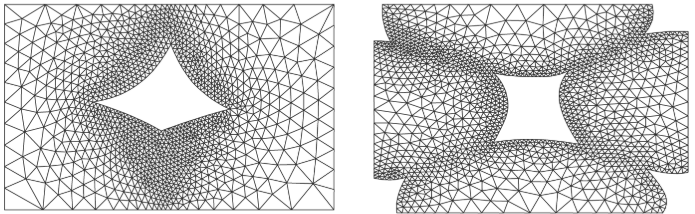
\includegraphics[width=1\textwidth]{chapter_2/figures/RVErodriguez.PNG}
    %\caption{Meshed RVE by Rodriguez}
    %\cite{Rodriguez2003MechanicalModeling}
    %\label{fig:RVERodriguez}
%\end{figure}

%He chose this unit cell to have a cavity surrounded by four roads, which would have the total surface of one road. After a convergence study of the FEM solution the appropriate mesh size was chosen to be 900 nodes for the aligned configuration and 1900 for the skewed configuration. The effective elastic properties  obtained from the simulation and experimentally tested samples where relatively similar, with less than 10 percent difference between experimental and calculated values in general. Larger negative differences occur for the Poisson ratio prediction. Rodriguez claims that it is pertinent to mention that results from the homogenization theory predict the material to be mono-clinic (one plane of material symmetry instead of orthotropic materials that differ along three mutually-orthogonal axis) instead of orthotropic as was originally assumed for the modeling. He implements tetrahedral elements for his mesh in Abaqus.

%Somireddy had a similar approach but uses the theory behind the process parameters combined with his observations of produced micrographs. He considers the form of the roads as elliptical which is supported by Sun \cite{Sun2008}, and implements roads that are approximately twice as wide as thick since that would give a relatively good trade off between the mechanical properties of the part with respect to the build time. He implements, in contrast to Rodriguez, hexahedral elements for his mesh. The RVE is subject to six different strains, applied individually using periodic boundary conditions to determine the unknown elements in the constitutive matrix, C. The effect of the assumption of perfect bonding between adjacent fibers are perfect seem to be small, since the results from the analysis is similar to experimental findings. 

%The analysis of the fundamental mesotructure (cross section of $(YX)[0]_n$) gives a basis for further reference, therefor different approaches will be quickly discussed.
%Somireddy \cite{Somireddy2018DevelopmentFDM} \cite{Somireddy2017FlexuralStudy} \cite{Somireddy2017MechanicalMesostructure} assumes an elliptical form with a 10\% overlap for the regular process in Z and Y direction. 

%Sheth \cite{Sheth2017NumericalOrientation} has applied a similar method with the homogenization of a FEM analyzed RVE, but investigated 4*4 ovallic roads with a 0.08mm fillet (as can be seen in figure \cite{Sheth2017NumericalOrientation}). They were loaded in different directions and the elastic properties where determined.

%\begin{figure}[H]
%    \centering
%    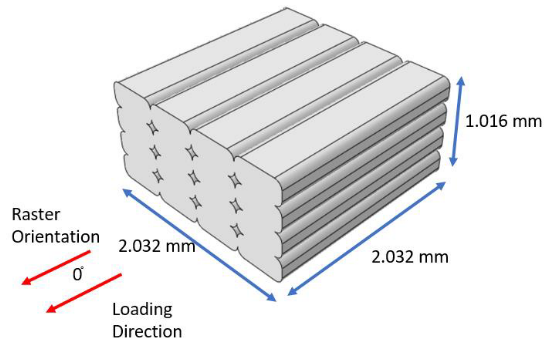
\includegraphics[width=0.5\textwidth]{chapter_2/figures/Sheth.PNG}
%    \caption{Meshed RVE by Sheth}
%    \cite{Sheth2017NumericalOrientation}
%    \label{fig:RVESheth}
%\end{figure}

%Recently (february 2019), Digimat presented a feature in its modelling software that includes a FE analysis that predicts the mechanical properties of a FFF RVE. They implement roads that are also ovalic in shape, and similar to the one used by Rodriguez. They even include a plastic region, which is relatively unique since no other researchers had introduced plasticity in their models. However, the current response is quite different from the experimental data (figure). Further experimentation should be done to analyze the possibilities of the Digimat software.  

%REST

%Alaimo also did strength!!! implement it 

%Following the 

%(Maybe last part from rodriguez)

%\subsubsection{Representative Volume Elements}
%review also this part
%If a solid has a periodic micro/mesostructure, a elasticity-based homogenization procedure can be used for determining the effective properties of a macroscopic part based on the properties of the meso/microscopic RVE or unit cell. The principle assumes that the periodicity of the material induces analogous periodic perturbation in the displacement, strain and stress fields. Rodriguez \cite{Rodriguez2003MechanicalModeling} implements a method known as the the asymptotic theory of homogenization. Homogenization is the procedure that relates the macroscopic variables to the microscopic variables through equation:
%\begin{equation}\label{homogenization}
%E(x)=\frac{1}{Y}\oint_\partial\frac{1}{2}[u(y)]\otimes n(y) +n(y)\otimes u(y)]dS
%\end{equation}%

%Where the prescribed macroscopic stress and strain tensors must be the average of the microscopic corresponding variables. 
%The solutions generated are the effective elastic properties described in the fourth order tensor $\bar{C}(x)$ of a macroscopic part composed out of mesoscopic unit cell of RVE's as is shown in figure \ref{fig:Homogenization}. He applies this approach on a perforated media which would simulate a FFF part. In figure \ref{fig:Homogenization} the RVE is seen to be orientated around one of the pores, which would result in a quarter of a road in each corner of the RVE. 

%\begin{figure}[H]
    %\centering
    %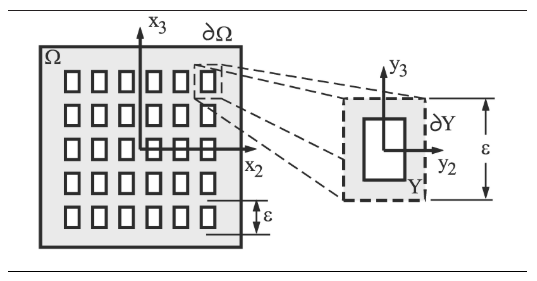
\includegraphics[width=0.5\textwidth]{chapter_2/figures/Homogenization.PNG}
    %\caption{Periodic body and unit cell (RVE)}
    %\cite{Alaimo2017InfluenceParts}
    %\label{fig:Homogenization}
%\end{figure}

%To find the elastic properties of the RVE one could use the Finite Element Method which is described in the following chapter (\ref{FiniteElementMethod}. The drawbacks of this method are the lack of plastic response (one could consider this insignificant since FFF parts have a limited  plastic response as can be seen in figure \ref{fig:Rodriguezgraph} and the assumption that there is perfect bonding between roads.
%Apart from Rodriguez, Sheth \cite{Sheth2017NumericalOrientation} has investigated the homogenization method implemented in BSAM to model the interface bond strength between adjacent raster roads for different orientation. This gave best results for a 0 degree raster or orientation (2\% deviation) and as much as 10\% for 45 and 90 degree angles. 
%Lui and Shapiro \cite{Liu2016HomogenizationStructures} proposed a new approach to find the elastic moduli for the part fabricated by FFF, using Green's function. 

%In the homogenization method used in Somireddy's work \cite{Somireddy2018DevelopmentFDM} a RVE is treated as a macroscopically homogeneous orthotropic material. He used a similar method to Melro to homogenize the RVE. Somireddy however, took different sizes of RVE's based on  elliptical road geometry in different directions.